\newpage
\section{Corpo rigidio}
Descriviamo un corpo rigido come un sistema di punti materiali, le distanze tra
i quali sono constati nel tempo. Punti: 
$$\{\vec{r}_{\alpha=1}^N\} \hspace{15pt} \{m_{\alpha}\}_{\alpha=1}^N \hspace{15pt} d_{\alpha\beta} = ||\vec{r}_{\alpha}(t) - \vec{r}_{\beta}(t)|| = const$$
Le leggi orarie $\vec{r}_{\alpha}(t)$ dei punti del sistema sono vincolate da questa condizione. Detto ciò invece di 3N coordinate indipendenti
ne bastano 6: $\vec{r}_{CM}(3)$ e 3 angoloi. Per il moto planare: $\vec{r}_{CM}(2)$ e 1 angolo.\\\\
Un punto geometrico determinato solo dalle posizioni $\vec{r}_{\alpha}$, come il centro di massa, ha pure distanze constante da tutti gli $\vec{r}_{\alpha}$, quindi $||\vec{r}_{CM} - \vec{r}_{\alpha}(t)|| = const$.
Si dice che tale punto è \textbf{solidale} al corpo rigido.\\\\
Due punti $\vec{r}_1(t), \vec{r}_2(t)$ solidali al C.R. definiscono un \textbf{vettore solidale} $\vec{r}_2(t) - \vec{r}_1(t)$. Conviene introdurre
un sistema di \textbf{assi solidali}, $\hat{x}', \hat{y}', \hat{z}'$ in cui le coordinate dei vettori solidali sono costanti.\\\\
In Geometrica planare (quella che usiano in questo corso):
\begin{figure}[h!]
    \centering
    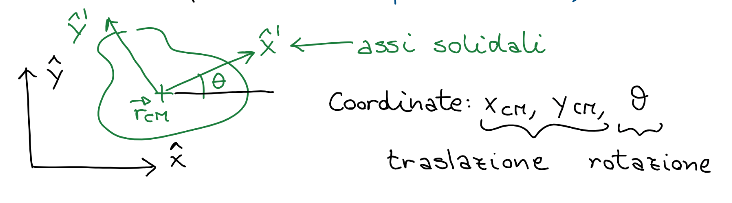
\includegraphics[width=0.65\textwidth]{images/geo-planare.png}
\end{figure}

\hspace{-15pt}Nella Geometria 3D (angoli di eulero):
\begin{figure}[h!]
    \centering
    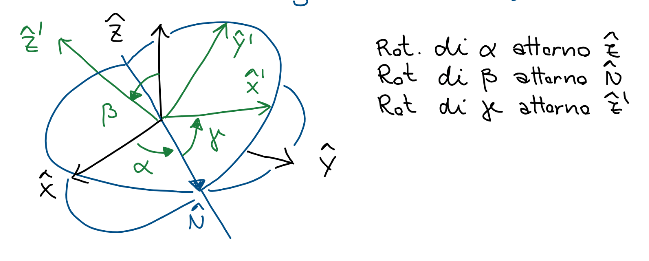
\includegraphics[width=0.55\textwidth]{images/geo-3d.png}
\end{figure}

\subsection{Teorema fondamentale sul moto del corpo rigido}
Il teorema fondamentale sul moto del corpo rigido dice che:
\begin{theorem}
    Ad ogni istante di tempo esiste ed è unico il vettore $\vec{w}(t)$, detto \textbf{vettore velocità angolare}, tale che, dati due punti qualunque $P_1, P_2$
    solidali al C.R.
    $$\dot{\vec{r}}_2(t) = \dot{\vec{r}}_1(t) + \vec{w}(t) \times [\vec{r}_2(t) - \vec{r}_1(t)]$$
    Dove $\vec{w}(t)$ è lo stesso per tutti i punti.
\end{theorem}
\hspace{-15pt}Sviluppiamo la teoria in modo generale, ma in questo corso incontriamo solo i moti planari dove:
$$\vec{r}_{\alpha}(t) = x(t) \hat{x} + y(t)\hat{y} + 0 \cdot \hat{z} \Rightarrow \vec{w}(t) = w(t) \hat{z}$$
\begin{example}
    $t= t_0, \vec{w}(t_0) = w\hat{z}, \dot{\vec{r}}_1(t_0) = v_0\hat{x}$
    $$\dot{\vec{r}}_2(t_0) = v_0\hat{x} + w\hat{z}x[L\hat{x}+ L\hat{y}] = v_0\hat{x} + wL\hat{y} - wL\hat{x} = (v_0 - wL)\hat{x} + wL\hat{y}$$
\end{example}
\begin{observation}
    Il vettore velocità angolare descrive il moto rotatorio del corpo rigido. Vogliamo quindi ottnere una equazione del moto per $\vec{w}(t)$ a partire dalla 2a Eq. 
    cardinale. Svolgiamo i passi necessari in questa lezione e nella prossima.
\end{observation}

\subsection{Momento angolare del corpo rigido}
Il momento angolare del corpo rigido si descrive come:
$$\vec{L}_p = M(\vec{r}_{CM}(t) - \vec{r}_p(t)) \times \dot{\vec{r}}_{CM}(t) + \sum_{\alpha=1}^{N}m_{\alpha}\vec{r}_{\alpha}'(t) \times \dot{\vec{r}}_{\alpha}'(t)$$
Con $M(\vec{r}_{CM}(t) - \vec{r}_p(t)) \times \dot{\vec{r}}_{CM}(t)$ dal CM. Mente $\vec{L}_{CM}(t) \equiv \sum_{\alpha=1}^{N}m_{\alpha}\vec{r}_{\alpha}'(t) \times \dot{\vec{r}}_{\alpha}'(t)$ rispetto al CM
\begin{equation*}
    \begin{split}
        \vec{L}_{CM}(t) & = \sum_{\alpha=1}^{N}[\vec{r}_{\alpha}(t) - \vec{r}_{CM}(t)] \times [\dot{\vec{r}}_{\alpha}(t) - \dot{\vec{r}}_{CM}(t)] = \sum_{\alpha=1}^{N} m_{\alpha}[\vec{r}_{\alpha}(t) - \vec{r}_{CM}(t)] \times [\vec{w}(t) \times [\vec{r}_{\alpha} - \vec{r}_{CM}(t)]]\\
                        & = \sum_{\alpha=1}^{N}m_{\alpha}[\vec{r}_{\alpha}'(t) \cdot \vec{r}_{\alpha}'(t)] \vec{w}(t) - \sum_{\alpha=1}^{N} m_{\alpha} \vec{r}_{\alpha}'(t)[\vec{r}_{\alpha}'(t) \cdot \vec{w}(t)]\\
                        & = \sum_{\alpha=1}^{N}m_{\alpha} 
                        \begin{pmatrix}
                            y_{\alpha}'^2 + z_{\alpha}'^2 & -x'_{\alpha} y'_{\alpha} & -x'_{\alpha}z'_{\alpha} \\
                            -y'_{\alpha}x'_{\alpha} & x_{\alpha}'^2 - z_{\alpha}'^2 & -y'_{\alpha}z'_{\alpha} \\
                            -z'_{\alpha}x'_{\alpha} & -z'_{\alpha}y'_{\alpha} & x_{\alpha}'^2 + y_{\alpha}'^2 
                        \end{pmatrix}
                        \begin{pmatrix}
                            w_{x'}(t)\\
                            w_{y'}(t)\\
                            w_{z'}(t)
                        \end{pmatrix}
    \end{split}
\end{equation*}
Coordinate nella base solidale: costante J.\\\\
La matrice J viene chiamata \textbf{tensore di inerzia} ed è una proprietà del corpo rigido, come la massa o il volume. $[J] = kg \cdot m^2$.
In 3D devo usare una matrice di rotazione con gli angoli di Eulero $w_{x'}, w_{y'}, w_{z'}$. Per moti planari (questo corso) $\vec{L}_p, \vec{L}_{CM}, \vec{w} // \hat{z}$
$$\vec{L}_{CM}(t) = \sum_{\alpha=1}^{N}m_{\alpha}(x_{\alpha}'^2 + y_{\alpha}'^2)w(t) \hat{z}$$
La parte $\sum_{\alpha=1}^{N}m_{\alpha}(x_{\alpha}'^2 + y_{\alpha}'^2)$ è detta $I_{CM}$ che sta per il momento di inerzia assiale. 
\begin{example}
    $I_{CM} = m_1|x_1'|^2 + m_2|x_2'|^2$ (ricordare che per la definizone $m_1x_1' + m_2x_2' = 0$)
\end{example}
\begin{example}
    Momento di inerzia assiale di un cilindro. $V= \pi R^2\cdot h \hspace{10pt}$ densità $\rho = M/V$
    $$I_z = \sum_{\alpha=1}^{N}m_{\alpha}(x_{\alpha}'^2 + y_{\alpha}'^2) = \int dm(x'^2 + y'^2) = \int dx' \int dy' \int_{0}^{h}dz' \cdot \rho(x'^2 + y'^2)$$
    Cambio di variabili nell'integrale per avere estremi più semplici: $x' = r \cdot \cos\Theta, y' = r \cdot \sin\Theta, dx' \cdot dy' = dr \cdot d\Theta \cdot r$
    $$= \int_{0}^{R}dr' \int_{0}^{2\pi}d\Theta' \cdot r'\int_{0}^{n}\cdot \rho \cdot r'^2 = \rho \cdot 2\pi \cdot h \cdot \frac{R^4}{4} = M\frac{1}{\pi R^2 h} \cdot 2\pi \cdot h \cdot \frac{R^4}{4} = \frac{1}{2}MR^2$$
    Posso calcolare il momento di inerzia assiale usando un punto solidale al C.R. diverso dal CM.
    \begin{equation*}
        \begin{split}
            I_p & = \sum_{\alpha=1}^{N}m_{\alpha}||\vec{r}_{\alpha} - \vec{r}_p(t)||^2 = \sum_{\alpha=1}^{N} m_{\alpha} ||\vec{r}_{\alpha}(t) - \underline{\vec{r}_{CM}(t) + \vec{r}_{CM}(t)} - \vec{r}_p(r)||^2\\
                & = \sum_{\alpha=1}^{N} m_{\alpha}\{||\vec{r}_{\alpha}(t) - \underline{\vec{r}_{CM}(t)}||^2 + ||\underline{\vec{r}_{CM}(t)} - \vec{r}_p(t)||^2 + 2[\vec{r}_{\alpha}(t) - \underline{\vec{r}_{\alpha}(t)}] \cdot [\underline{\vec{r}_{CM(t)} - \vec{r}_p(t)}]\}\\
                & = I_{CM} + M \cdot ||\underline{\vec{r}_{CM}(t)} - \vec{r}_p(t)||^2 + 2\underline{\{\sum_{\alpha=1}^{N}m_{\alpha}[\vec{r}_{\alpha}(t) - \vec{r}_{CM}(t)]\} \text{ (= 0) }} \cdot [\underline{\vec{r}_{CM}(t)} - \vec{r}_p(t)] \Rightarrow I_p = I_{CM} + M||\vec{r}_p||^2
        \end{split}
    \end{equation*}
    \underline{Teorema degli assi paralleli (Hyuhens - Steuiner)}
\end{example}

\begin{example}
    Cilindro con foto parallelo all'asse. Considero due cilindri fittizi di densità uguale al cilindro 1. Il 2 
    occupa lo spazio del foro, il 3 come 1 ma senza foto.
    $$            
    I_1^{(3)} = I_1^{(1)} + I_1^{(2)} \text{ (per additività del momento di interzia) } = I_1^{(1)} + I_1^{(2)} + M^{(2)} \cdot d^2\\
    $$
    \begin{equation*}
        \begin{split}
            I_1^{(1)} & = I_1^{(3)} - I_2^{2} - M^{(2)} d^2 = \frac{1}{2}(\rho v^{(3)})R^2 - \frac{1}{2}(\rho v^{(2)})R_2^2 - (\rho v^{(2)})d^2\\
                      & = \frac{1}{2}\rho h \pi((R^4) - R_2^4 - R_2^2 d^2) \:\:\:\:\underline{(g=\frac{M}{\pi R^2h})} \:\:\:\:= \frac{1}{2}MR^2[1 - \frac{R_2^4}{R^2} - \frac{R_2^2d^2}{R^4}] < \frac{1}{2}MR^2
        \end{split}
    \end{equation*} 
\end{example}
\hspace{-15pt}Equazioni cardinali per il corpo rigido:
$$
I. \:\: \ddot{M}\vec{r}_{CM}(t) = \sum_{i}\vec{F}_i(e)(t)
$$
Non importa il punto di applicazione delle forte \textbf{esterne} $\vec{F}_i^{(E)}(t)$
$$
II. \:\: \frac{d}{dt}[I_z\omega(t)\hat{z} + M[\vec{r}_{CM} - \vec{r}_p(t)] \times \dot{\vec{r}}_{CM}] = \sum_{i}[\vec{r}_i(t) - \vec{r}_p(t)] \times \vec{F}_i^{(E)}(t) - M\dot{\vec{r}}_p  \times \dot{\vec{r}}_{CM} 
$$
La parte $I_z\omega(t)\hat{z}$ è una forma semplificata valida solo per il modo nel piano $\hat{x}, \hat{y}$. Essenziale il punto di applicazione delle forze.
Polo $\vec{r}_p$ arbitrario, scelgo quello che semplifica.

\begin{example}
    Cilindro vincolato e forza costante. \\
    Scelto come polo il CM. $\vec{F} = - F\hat{x} \:\:\: \vec{N}= N \hat{x} \:\:\: \vec{\omega} = \dot{\Theta}\hat{z}$.\\
    Abbiamo che $N = F$ e nessuna info su $\Theta$. I vincoli sono: $\vec{r}_{CM}(t) \equiv 0 \Rightarrow \ddot{\vec{r}}_{CM}(t) = 0$
    \begin{itemize}
        \item $I. \:\: M\ddot{\vec{r}}_{CM} = \vec{F} + \vec{N} = (N - F)\hat{x}$
        \item $II. \:\: \frac{d}{dt}[I_z\omega(t)\hat{z} + M[\vec{r}_{CM}(t) - \vec{r}_p(t)] \times \dot{\vec{r}}_{CM}] = \sum_{i}[\vec{r}_i(t) - \vec{r}_p(t)] \times \vec{F}_i^(E)(t) - M\dot{\vec{r}}_p \times \dot{\vec{r}}_{CM}$
    \end{itemize}
    $$I_z\dot{\omega}(r)\hat{z} = (\vec{r}_i - \vec{r}_{CM}) \times \vec{F} + (\vec{r}_{CM} - \vec{r}_{CM}) \times \vec{N} = R\hat{y} \times (-F\hat{x}) + 0 = RF\hat{z} \Rightarrow I_z\ddot{\Theta}(t) = RF \hspace{10pt}\ddot{\Theta} = \frac{2F}{MR} \text{ costante}$$
\end{example}

\subsection{Condizione del "puro rotolamento"}
Il punto $\vec{r}_1$ del corpo rigido a contatto con la superficie al tempo $t_1$ è fermo. Al tempo 
$t_2$ un altro punto $\vec{r}_2$ del corpo rigido è a contatto con la superfice. Il punto geometrico $\vec{r}_C(t)$ di contatto 
\textbf{non è solidale} e il suo moto non è determinato dal vettore $\vec{w}(t)$
\begin{figure}[h!]
    \centering
    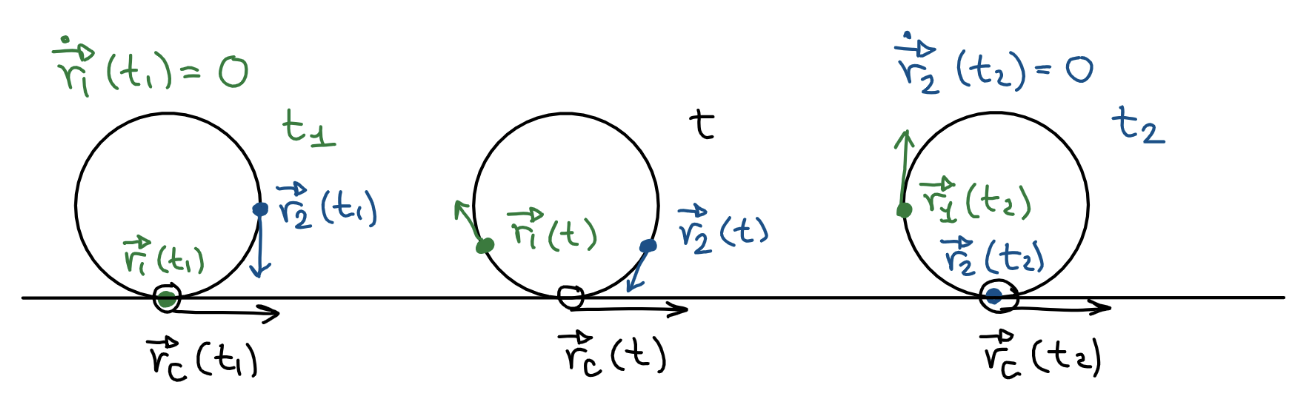
\includegraphics[width=0.65\textwidth]{images/puro-rotolamento.png}
\end{figure}
\begin{example}
    Cilindro trainato su piano scabro.
    \begin{figure}[h!]
        \centering
        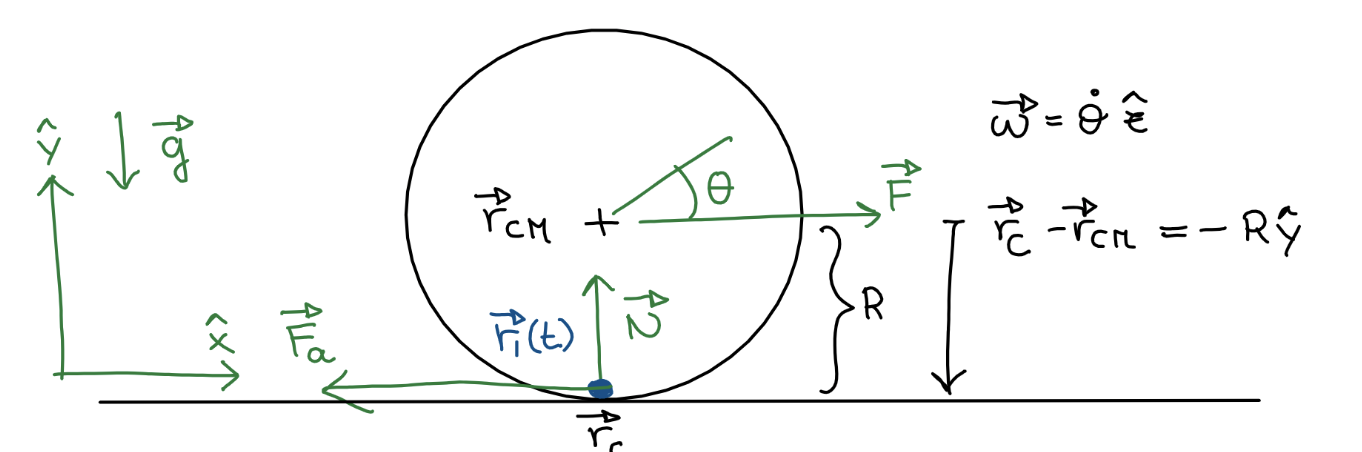
\includegraphics[width=0.50\textwidth]{images/cilindro-trainato-piano-scabro.png}
    \end{figure}
    \begin{itemize}
        \item $I. \:\: O = M\ddot{y}_{CM}(t) = -Mg + N \Rightarrow N = mg \hspace{15pt} M\underline{\ddot{x}_{CM}} = F - F_a$
        \item $II. \:\: I_z\underline{\dot{\omega}(t)}\hat{z} = (\vec{r}_{CM} - \vec{r}_{CM}) \times \vec{F} + (\vec{r}_{CM} - \vec{r}_CM) \times (\vec{F}_a + \vec{N}) = 0 + (-R\hat{y}) \times (-F_a\hat{x} + N\hat{y}) = -RF_a\hat{z}$
    \end{itemize}
    \underline{Abbiamo 3 incognite}.
\end{example}
\hspace{-15pt}Vincolo del puro rotolamento
$$0 = \dot{\vec{r}}_{CM}(t) + \vec{\omega} \times [\vec{r}_c(t) - \vec{r}_{CM}(t)]$$
Ma quando il punto $\vec{r}_1$ è a contatto $\vec{r}_1(t) = \vec{r}_C(t) \Rightarrow 0 = \dot{\vec{r}}_{CM}(t) + \vec{\omega} \times [\vec{r}_C(t) - \vec{r}_{CM}(t)]$ 
$$ = \dot{x}_{CM}(t)\hat{x} + \dot{\Theta}(t)\hat{z} \times (-R\hat{y}) = \dot{x}_{CM}(t)\hat{x} + R \dot{\Theta}(t)\hat{x} \Rightarrow \underline{\dot{x}_{CM}(t) = -R\dot{\Theta}(t)} \Rightarrow \ddot{x}_{CM}(t) = -R\ddot{\Theta}(t)$$
Sostituisco nelle equazioni cardinali
$$
\begin{cases}
    -MR\ddot{\Theta} = F - F_a\\
    \frac{1}{2}MR^2 \ddot{\Theta} = -RF_a
\end{cases}
\:\:\:
\begin{cases}
    F_a = -\frac{1}{2}MR\ddot{\Theta}\\
    -MR\ddot{\Theta} = F + \frac{1}{2}MR\ddot{\Theta}
\end{cases}
\begin{cases}
    \ddot{\Theta} = -\frac{2}{3}\frac{F}{MR}\\
    F_a = \frac{1}{3}F
\end{cases}
$$
Minimo $\mu_s$ per mantenere puro rotolamento?
$|F_a| \leq \mu_S|N| \hspace{15pt} \mu_S \geq \frac{F/3}{Mg} = \mu_s,min$

\subsection{Energia del corpo rigido}
$$K(t) = \frac{1}{2}M||\dot{\vec{r}}_{CM}(t)||^2 + \sum_{\alpha=1}^{N}\frac{1}{2}m_{\alpha}||\dot{\vec{r}}_{\alpha}'(t)||^2$$
Con $\frac{1}{2}M||\dot{\vec{r}}_{CM}(t)||^2$ dal CM e $\sum_{\alpha=1}^{N}\frac{1}{2}m_{\alpha}||\dot{\vec{r}}_{\alpha}'(t)||^2$ rispetto al CM $\equiv K_{CM}(t)$